% Chapter Template

\chapter{Quantum Dots} % Main chapter title

\label{sec:Quantum_Dots} % Change X to a consecutive number; for referencing this chapter elsewhere, use \ref{ChapterX}

%----------------------------------------------------------------------------------------
%	SECTION 1
%----------------------------------------------------------------------------------------

\section{Fundaments}

A quantum dot (QD) existentially a small ``box'' filled with particles. When the size of this region is comparable to the wavelength of the particle that populates it, the system becomes quasi 0-dimensional, exhibiting a discrete energy spectrum. This is somehow similar to an atoms, and this is why QD's are usually called artificial atoms. The dots can be filled with electrons or holes, depending on which atoms the substrate is doped with. Different sites can be coupled via tunnel barriers, allowing the particles to ``jump'' from one dot to another. It is also common to couple a source and a drain reservoir that enable the exchange of particles. By attaching current and voltage probes to these reservoirs we can measure the electronic properties of the device. This description of a QD is very general, and this is why exist systems of may different sizes and materials. For instance self-assembled quantum dots, semiconductor lateral and vertical dots, or even carbon nanotubes. An example of this devices can be found in Fig.~\ref{fig:different_devices}. In this work, we focus on lateral gated semiconductor quantum dots. These devices allow a great control over the different parameters of the system, what can be used to tune it's values in situ. 
\begin{figure}[!htb]
	\centering
	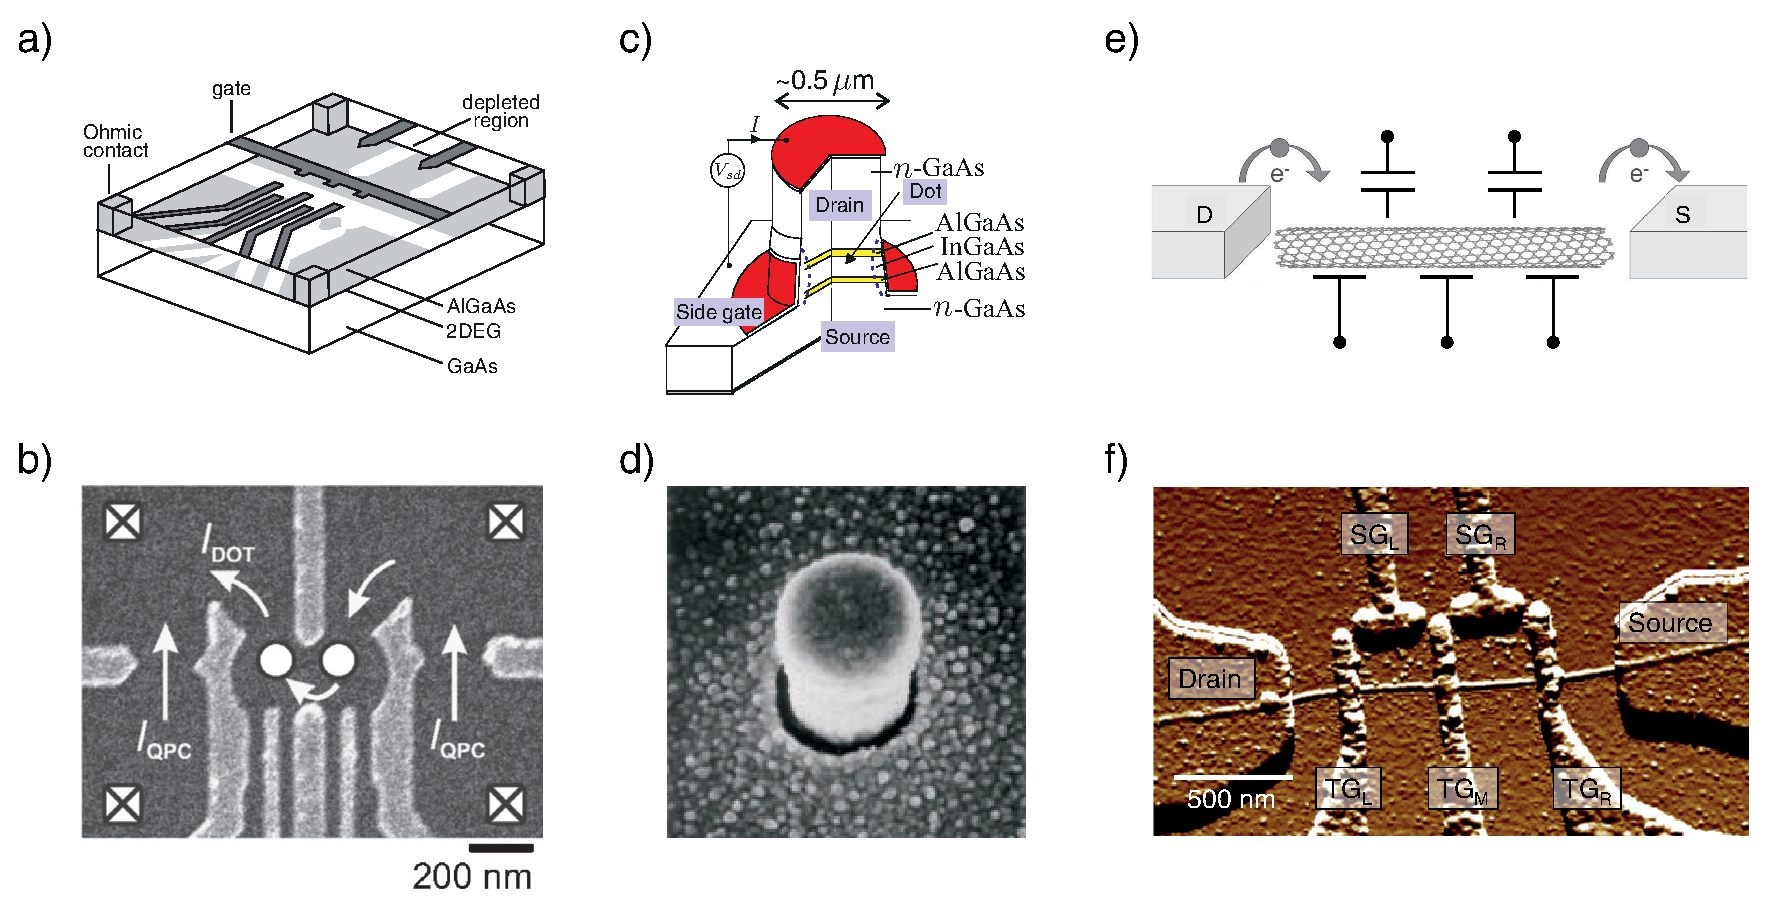
\includegraphics[width=\linewidth]{different_devices.eps}
	\caption{Different devices for quantum dots. a) Schematic view and b) scanning electron micrograph (SEM) of a lateral DQD, taken from ref. \cite{Hanson2007}. c) Schematic and d) SEM images of a vertical semiconducting QD, taken from ref. \cite{Kouwenhoven2001}. e) Schematic and f) atomic force microscope (AFM) of a DQD implemented in a carbon nanotube, taken from e) ref. \cite{SapmazPhd} and f) ref. \cite{Sapmaz2006}.}
	\label{fig:different_devices}
\end{figure}

Fabrication of gated quantum dots starts with a layered heterostructure composed by different semiconducting materials. A common choice for the semiconductors is GaAs and AlGaAs grown on top of each other. By doping the n-AlGaAs with Si we can introduce free electrons, which are accumulated in the interface forming a 2-dimensional electron gas (2DEG) \cite{Elzerman2005}. If we are interested in holes instead of electrons we can keep the GaAs/AlGaAs heterostructure undoped \cite{Tracy2014}. By applying negative voltages to metal surface electrodes (gates) on top of the semiconductor heterostructure the 2DEG is locally depleted, thereby forming the QD. In order to control the electrostatic potential of the dots with respect to the reservoirs we can couple it capacitively to a gate electrodes. The tunneling rate can be also modified with electric fields applied to the gates located between neighbouring dots. With this we have an all-electrical control over the system. We can also use a magnetic field to produce a Zeeman splitting in the spin of the particles.

\section{Transport}
The charge transport thought the system is a perfect way to measure the state of the device, since the intensity observed depends on the states of the particles inside the quantum dots. in the contacts (source and drain) there are free particles with energies up to the chemical potential $\mu$. At low temperatures this chemical potential corresponds to the Fermi energy. During the entire chapter we will consider that the temperature of the device is low enough so the approximation of the chemical potential as a step function is justified. Applying a voltage difference between the two reservoirs known as the bias voltage $V_{\text{bias}}$. The relation between this three parameters is
\begin{equation}
	V_{\text{bias}}=\frac{\mu_R-\mu_L}{e}\; ,
	\label{eq:deff_bias}
\end{equation}
where $L$ and $R$ denote the left and right contact respectively, and $e$ is the electron charge. The choice of the sign is a convention, different choices can be found in the literature. The chemical potential for the quantum dots is defined as the required energy to add a new particle in the site. The more particles there are in the QD, the higher is the chemical potential, thus forming what is known as the electrochemical ladder. All this discrete levels can be shifted by the gate voltage $V_G$. This is depicted in Fig.~\ref{fig:potential_ladder}. If the chemical potential of a reservoir ir larger than $\mu(N)$, then one particle can enter in the quantum dot. This will occur until the QD's potential reaches a value higher than the contact $\mu(N+1)>\mu_i$. The same thing will happen in reserve, if $\mu(N)>\mu_i$, the particles will leave the system towards the reservoir until a balance is reached. In the example shown two particles can enter initially in the QD from the right reservoir, but only one of then can tunnel out to the left drain. Then a net intensity of one particle will flow continuously from right to left.
\begin{figure}[!htb]
	\centering
	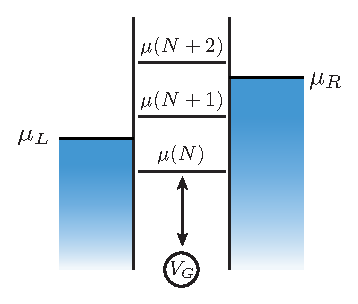
\includegraphics[width=0.4\linewidth]{potential_ladder.eps}
	\caption{Sketch of the electrochemical ladder in a quantum dot. The energy origin is given by the gate voltage $V_G$.}
	\label{fig:potential_ladder}
\end{figure}

In order to know exactly the number of particles inside the devices we must use the stability diagrams. This kind of measures can be obtained by two different techniques, but with very similar results. In both of them the chemical potential of the reservoirs are keep constant and equal to each other, that is $V_{\text{bias}}=0$. Then the gate voltages of each dot are modified independently, trying to map out as much of the area as possible. The aim of these measures is to obtain at which values fir the gate voltages there is a variation in the number of particles. One possibility for this is the use of a quantum point contact (QPC), which is sensitive to the variation of charge inside the QD. On the other hand, we can determine this movement of the particles also via the charge intensity. Both methods assume a sequential tunneling, that is, only one particle enter or exit the device at each time, so every time a transition is measured, either with the QCP or with the electronic intensity, we can assure that only one particle has changed its position. Once we don't see any more transitions all the QD's are empty, allowing us to define the exact number of particles for each quantum dot in each region. In Fig.~\ref{fig:stability_diagrams} we can shown the results for these two techniques applied to the same double quantum dot. The fact that the ``honeycomb'' are formed by lines with certain slope is due to the capacitively coupling, changing $V_R$ will not only affect the right dot but has a small contribution on the other points.
\begin{figure}[!htb]
	\centering
	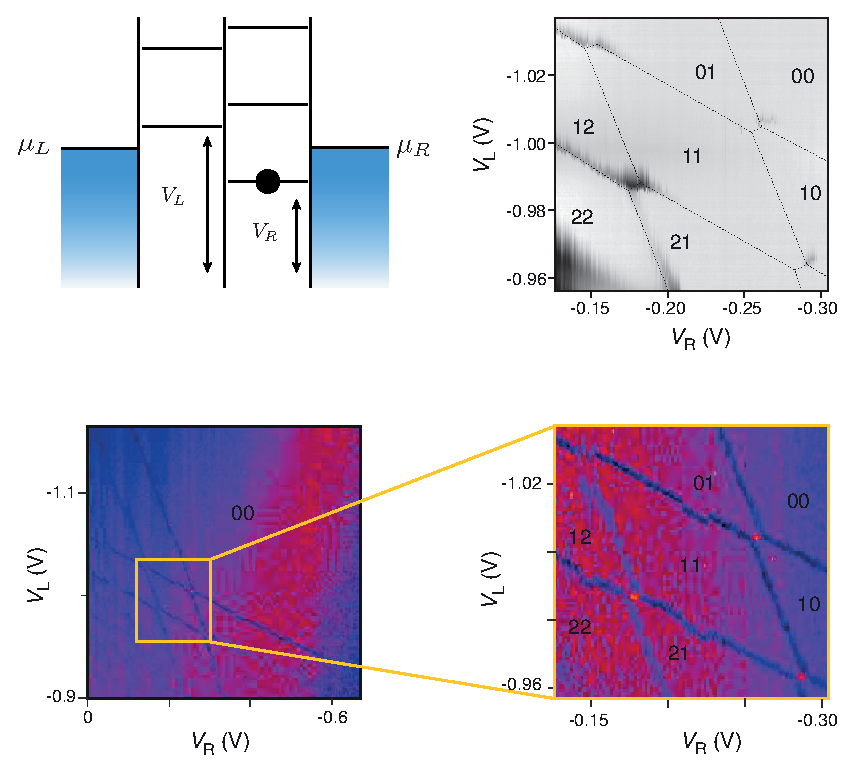
\includegraphics[width=0.8\linewidth]{stability_diagrams.eps}
	\caption{a) Sketch of a DQD with one particle in the right dot, or what in the same, in the region 01. b) and c) measures of the stability diagram of the same GaAs DQD sample via b) charge intensity and c) differential intensity of a QPC $dI_{\text{QPC}}/dV_L$. Both diagrams are taken form ref. \cite{Elzerman2003}.}
	\label{fig:stability_diagrams}
\end{figure}

Once we know in what region we are working, we must have some techniques to measure the state of the QD's. In the next sections we define some widely used techniques used for single, double and triple qubits.

\subsection{Coulomb Blockade}
Now imagine a system of a single quantum dot in which the bias voltage has a non-vanishing value $V_{\text{bias}}\neq 0$. As we change the gate voltage, at some values the chemical potential will lie within the window between the two reservoirs, e.g $\mu_R>\mu(N)>\mu_L$. At this point a particle can tunnel from the right reservoir to the QD, and then exit the system again through the left contact, so a net current will flow thought the system. On the contrary, in the chemical potential of the is outside the windows, then no particle can enter or leave the point, so the measured current will eventually vanish. Both scenarios are represented schematically in Fig.~\ref{fig:coulomb_diamonds}~a) with green and red dots respectively. This behaviour is known as the Coulomb blockage, and mapping the gate-bias voltage plane we obtain the so-called Coulomb diamonds Fig.~\ref{fig:coulomb_diamonds}~b). If the measurements are made at a finite temperature, the Fermi distribution acquire a smooth shape and even if the chemical potential of the dot is outside the windows, the particles can tunnel in or out the system thanks to the thermal phonons interchanged with the vibrations of the lattice. This translate into diffuse boundaries for the Coulomb diamonds.
\begin{figure}[!htb]
	\centering
	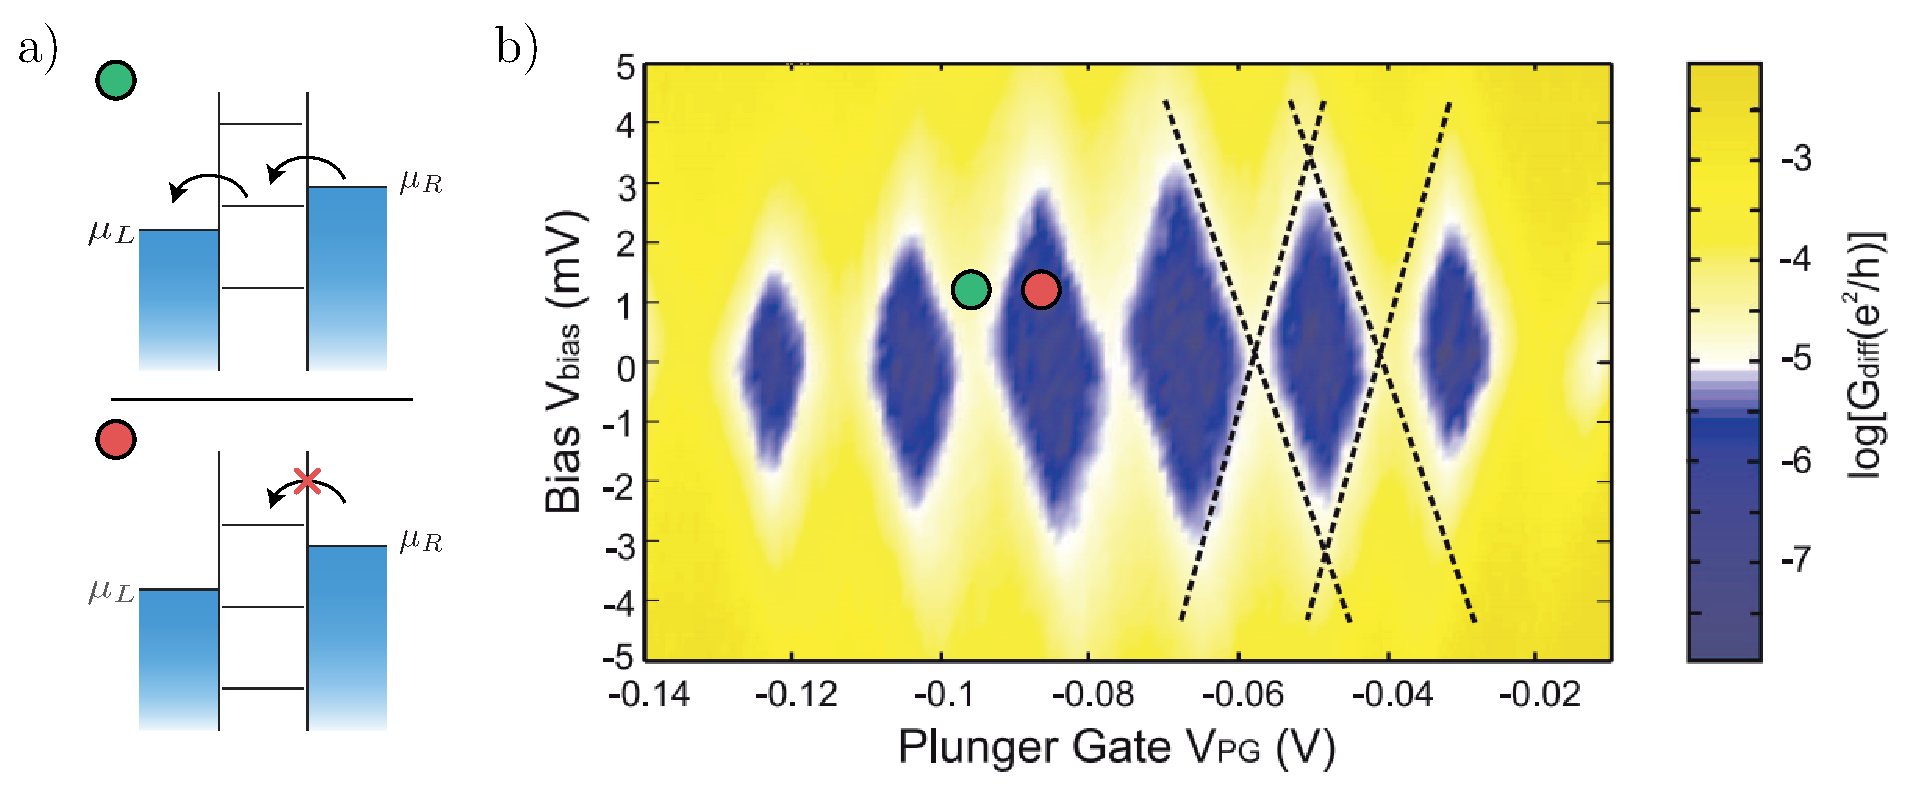
\includegraphics[width=\linewidth]{coulomb_diamonds.eps}
	\caption{a) Schematic images shown the case of Coulomb blockage (red) and non-vanishing intensity (green). b) Coulomb diamonds measured in a graphene QD, figure taken from ref. \cite{Stampfer2008}.}
	\label{fig:coulomb_diamonds}
\end{figure}

\subsection{Pauli Blockade}
For the moment the spin of the particles plays no important role in the measurement, this is because no magnetic field was applied and the energy levels was degenerated. Thanks to the Zeeman splitting we can lift this degeneracy. Imagine a DQD system in which we have confined one particle with a given spin, up for instance. We will work in the region in which one more particle can enter the system. In this kind of systems the intradot energy use to be high enough, so we consider just one orbital per QD. That is, two particle can only occupy the same site in their spines are antiparallel, in what is called the double occupation singlet. For future references to this state we will use the notation S(2,0) if the two particles are in the left dot or S(0,2) if there are in the right dot. There are four more possible states corresponding to the single occupation singlet and the three possible triplets with different total spin. All together form a complete basis for a DQD system populated with two particles,
\begin{equation}
	\begin{split}
	\ket{S(0,2)}&=\ket{0,\uparrow\downarrow}\\
	\ket{S(2,0)}&=\ket{\uparrow\downarrow,0}\\
	\ket{S(1,1)}&=\frac{1}{\sqrt{2}}\left[\ket{\uparrow,\downarrow}-\ket{\downarrow,\uparrow}\right]\\
	\ket{T_0(1,1)}&=\frac{1}{\sqrt{2}}\left[\ket{\uparrow,\downarrow}+\ket{\downarrow,\uparrow}\right]\\
	\ket{T_+(1,1)}&=\ket{\uparrow,\uparrow}\\
	\ket{T_-(1,1)}&=\ket{\downarrow,\downarrow}\;.
	\end{split}
	\label{eq:molecular_basis}
\end{equation}
In addition, we only allow the particles to tunnel from one dot to another conserving the spin projection, so the transition $\ket{\uparrow,0}\rightarrow\ket{0,\downarrow}$ is not possible for the moment. Returning to our system with one particle confined, that is, whose energy level is below the chemical potential of the two contacts, as an example let's locate this particle in the left QD. In the reservoirs there are both spin up and spin down particles, so in principle we can not choose which particle we want to enter in the system. We set the detuning between dots such that the energy of the states $S(2,0)$ and $T_+(1,1)$ in resonance. In this situation we can find two qualitatively behaviours for the system, which are depicted on the right hand side of Fig.~\ref{fig:pauli_blockade} a). If we apply a negative bias voltage, i.e. $\mu_L>\mu_R$ recall Eq.~(\ref{eq:deff_bias}), only a spin down particle can enter the system, which tunnel to the other dot and finally leaving the system thought the right contact. This situation gives a net charge intensity than can be measured (green dot). On the other hand, with $V_{\text{bias}}>0$ we have again two possibilities. If the particle that enters the system is antiparallel to the one that is confined on the left dot, then the first one can tunnel conserving its spin to later tunnel out to the left reservoir, what gives a measurable intensity. But if the particle that enter the system have spin up,  we are looking at a situation where the particle won't be able to move in any direction. We have said that double occupation tripled state $T_+(2,0)=(\uparrow\uparrow,0)$ is so high in energies that the particle can not reach it. We have also forbidden a spin-flip tunneling, so the double occupation singlet state is not an option. Lastly, if the right potential is high enough the particle can not tunnel back, allowing a particle with spin down to enter the system. In this scenario we have a steady system that presents no intensity (red dot). With this we have shown what is known as Pauli Blockage, which has been experimentally measured in a GaAs vertical DQD populated with electrons Fig.~\ref{fig:pauli_blockade} b).\\
\begin{figure}[!htb]
	\centering
	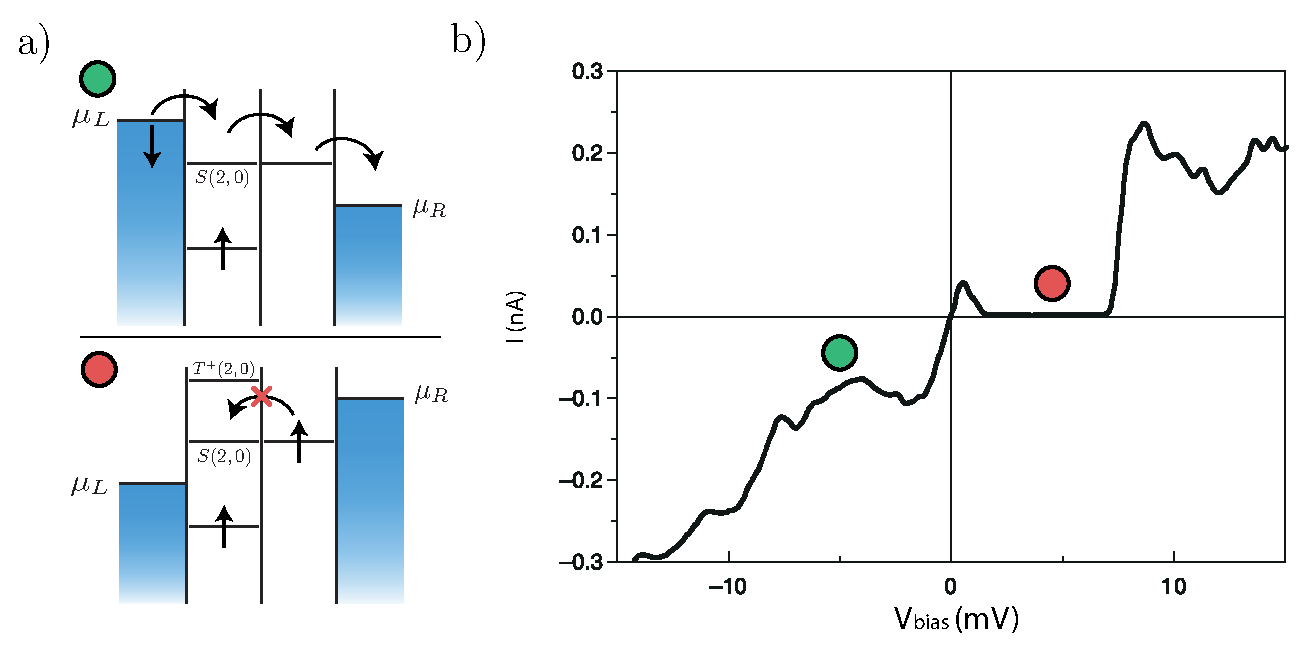
\includegraphics[width=\linewidth]{pauli_blockade.eps}
	\caption{a) Schematic representation of the Pauli blockade in a DQD. b) Experimental results obtained in a GaAs vertical DQD populated with electrons, figure taken from ref. \cite{Ono2002}.}
	\label{fig:pauli_blockade}
\end{figure}

This effect is crucial in order to measure the spin of the particle that we had confined initially in the system. We can apply electron spin resonance (ESR) techniques to rotate the spin of the particle, and measured the intensity when the system  is tuned in the Pauli blockade region. When the spin of the confined particle is rotated we can observe that the blockaded is lifted and intensity increase Fig.~\ref{fig:esr_detection}. This offers a possibility for the construction of a measurement quantum gate, as essential component in the development of quantum computing. In this figure we can observe one of the main difficulties when trying to encode a qubit in this systems, the decoherence and dephasing times. Both effects cause the damping  of the oscillations, thus restricting the number of operations we can do, while maintaining a given fidelity.
\begin{figure}[!htb]
	\centering
	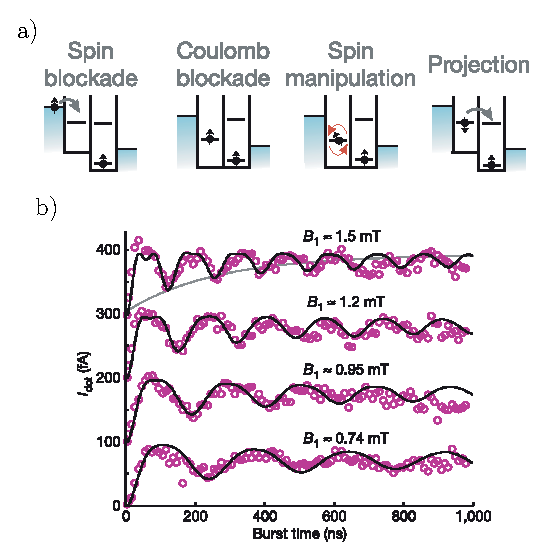
\includegraphics[width=0.7\linewidth]{esr_detection.eps}
	\caption{Use of the Pauli spin blockade to measure the spin of an electron in a GaAs lateral DQD. a) Protocol followed to initialize the system, make the ESR protocol and the final measurement of the spin. b) Experimental results for the intensity measured in terms of the total times of the applied pulse. The different curves correspond to different magnetic fields. Figures taken from ref. \cite{Koppens2006}.}
	\label{fig:esr_detection}
\end{figure}

\section{Quantum Gates with QD}

The main point for the study of quantum dots is the possibility to implement an universal set of quantum gates. In this section we will present two different approaches to this goal, obtaining in both of then universal gates of one and two qubits, with which any other conceivable gate can be achieved by combining this two operations. Here we will mention some adiabatic passage techniques which will be explained in more detail in Chapter~\ref{sec:Shortcuts_to_Adiabaticity}. The first work that we will mention have both theoretically and experimentally proven \cite{Petta2010,Ribeiro2009,Ribeiro2010} the viability to encode a qubit in the spin of a GaAs DQD populate with electrons, but not on the spin of the individual particle but in the singlet and triplet states, $\ket{S(2,0)}$ and $\ket{T_+(1,1)}$ respectively. In order achieve a one qubit gate the authors take advantage of the appearance of an anticrossing due to the hyperfine interaction. The computed energy spectrum of this system is plotted in Fig.~\ref{fig:electron_hyperfine} a).
\begin{figure}[!htb]
	\centering
	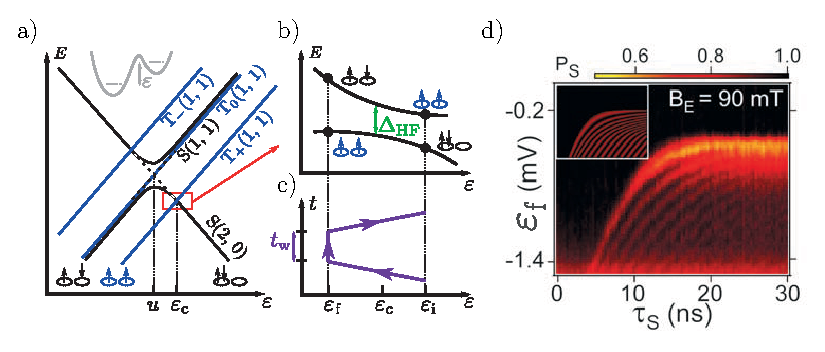
\includegraphics[width=0.8\linewidth]{electron_hyperfine.eps}
	\caption{a) Energy spectrum for a GaAs DQD as a function of the detuning $\varepsilon$. b) Zoom at the avoided crossing opened due to the hyperfine interaction of the electrons with nuclear spins. c) Dependence of the detuning with time used for the LZS interference. d) Experimental results for the probability of measure the singlet state $P_S$ as a function of the final detuning $\varepsilon_f$ and the total time of the protocol  $\tau_{s}$. Figures a), b) and c) taken from ref. \cite{Ribeiro2010}, d) taken from ref. \cite{Petta2010}.}
	\label{fig:electron_hyperfine}
\end{figure}

The protocol used consist in two consecutive passages thought the avoided crossing, among which there is a certain amount of time where the system is keep unchanged $t_W$ to acquire a relative phase between both states, Fig.~\ref{fig:electron_hyperfine} c). This protocol is known in the literature as a Landau-Zener-Stückelberg interferometry \cite{Shevchenko2010} (LZS). These passings can be easily achieve experimentally just by modifying the detuning between the dots. The authors opted to keep the theoretical computations as simpler as possible by choosing a linear dependence of the detuning with time. The hyperfine interaction is implemented as a semiclassical Overhauser field obtaining an effective Hamiltonian. With this it can be shown that the direction of rotation in the Bloch sphere and in angle can be tuned via the waited time between passaged and the slope of them. A two qubits CNOT gate can be implemented by joining two DQD in a lateral array. The interdot electron interchange energy affect the position at which the anticrossing is located, which in turn affects the result of the LZS. Experimentally the system in initialize in double occupation singlet state, and after the two passages the probability to remain in the singlet state is measured, Fig.~\ref{fig:electron_hyperfine} d). This study has two main problems when we try to implement it in a real life quantum gate, one of the is that the analytical solutions given are the result of a large number of approximations such as linearising the eigenenergies near the anticrossing or expanding up to first-order the solution for the dynamics of the system. This implies that when a certain rotation is need, the fidelity of the operation will be affected. The other disadvantage of this protocol is the population of the double occupation singlet state, what is the source of charge noise what reduce the QD's dephasing time \cite{Kuhlmann2013,Fujisawa2000}. This source of noise is what we will try to solve in Chapter \ref{sec:DQD} using holes instead of electrons.


